\documentclass{article}%
\usepackage[T1]{fontenc}%
\usepackage[utf8]{inputenc}%
\usepackage{lmodern}%
\usepackage{textcomp}%
\usepackage{lastpage}%
\usepackage{authblk}%
\usepackage{graphicx}%
%
\title{Heat Shock Protein 27 Is Spatially Distributed in the Human Placenta and Decreased during Labor}%
\author{Rodney Manning}%
\affil{Department of Minimally Invasive Surgery, The First Affiliated Hospital of Nanjing Medical University, Nanjing 210029, P.R. China}%
\date{01{-}01{-}2004}%
%
\begin{document}%
\normalsize%
\maketitle%
\section{Abstract}%
\label{sec:Abstract}%
This is an edited transcript of the audio.\newline%
You can see a lot more color inside. This is an important thing to note. Very good.\newline%
Now, I know what you're thinking. This isn't the old sick people who you're talking about. That's not quite what I'm saying, but you're probably thinking that.\newline%
Well, if I told you that at all, it would not have happened to me. My mother died years ago with the virus that keeps bloating me and keeping me in pretty bad shape. So it is not like she died before I did.\newline%
But what I'm trying to say is that for patients that have established infection with tuberculosis, more often than not, they don't exhibit the traditional symptoms of acute bronchitis that people tend to have. They don't have the usual things like headaches or dizziness or fatigue. They don't have trouble recognizing that they're coughing themselves up. They don't have the typical symptoms of some other lung infections. There's nothing to indicate anything wrong with them yet. It just doesn't happen. I did a lot of research and I knew nothing about this.\newline%
So to those patients, here's what you're going to understand: These antibodies act in two different ways. They're either blocks that can shut down parts of the bacteria that cause infection. When that happens, the bacterial flora that's there can take over and cause more trouble. A lot of times the labs that do the disease diagnosis actually destroy the bacteria that's present in the patients, killing any bacteria that weren't present in the patient when they received the diagnosis.\newline%
What do I mean by "all this stuff you're seeing" is that these signals are known as sporadically activated antibodies. I mean these are signals that get activated and I've described in past blogs that they are really special signals to trigger a condition. I think these are signs that any infection that's at all non{-}convincing could potentially cause me to be sick with the serious infections.\newline%
Basically, this means that these are not benign not{-}weilding antibodies. Not cases of milder infections where you don't show the usual normal symptoms. If you've got a problem with antibiotic resistance, the fact that they have activated them again is something that may be a sign that antibiotics can't be an effective against these organisms. So it really says a lot.\newline%
Let's talk about the disease. Aspergillus is a very tricky little disease to treat. It's not uncommon for people to have an infection with quite an aggressive form of severe disease. The problems with Aspergillus is not that you can't treat it with antibiotics, it's that it has infection with several different organisms that cause it. Aspergillus can produceand this is the troubleit makes you sick pretty much by itself.\newline%
So how do I explain the difference between mild versus severe cases of it? Most of the time, we just replace the antibiotics with another group of antibiotics. If you don't have that one group of antibiotics, we're going to throw a couple of the newer ones, again. But even though we see a result that is not contagious, there is a human microbe that actually lives next to the infected person. And that's called bacterium{-}infected brain.\newline%
There are two kinds of Aspergillus bacteria. One is called the genetic fingerprinting variant. This particular one is the one that really makes you sick. In all the people that have been treated with these two types of Aspergillus, the treatment works about 90 percent of the time. But in about 15 percent of the cases the one

%
\subsection{Image Analysis}%
\label{subsec:ImageAnalysis}%


\begin{figure}[h!]%
\centering%
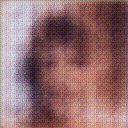
\includegraphics[width=150px]{500_fake_images/samples_5_366.png}%
\caption{A Close Up Of A Black And White Cat}%
\end{figure}

%
\end{document}